\documentclass[]{article}

%opening
\title{Planning and Risks}
\author{Exam Number: B032374}
\date{\today}

\usepackage[parfill]{parskip}
\usepackage{pgfgantt}
\usepackage{multicol}
\usepackage{tikz}
\usepackage{pgfplots}

\usepackage{graphicx}
\graphicspath{ {images/} }

\usepackage{amsmath}

\usepackage{booktabs}
\usepackage[font={small,it}]{caption}

\begin{document}

\maketitle

\section{Introduction}


Investigate the effect of activation function on a multi-layer neural network.

This part of the report investigates how the choice of activation function affectstraining set performance of a small multi-layer model. Three transformation functions withdifferent characteristics were tested and evaluated.
Additionally

How does the number of hidden layer and hidden units affect the training of a deep neural network?



\section{Methodology}

As the methodology used for the three experiments were similar, this section will cover the overall structure of the code and neural networks used throughout the investigation. Instead of building three isolated models and corresponding methods to run the experiments, some effort was put into building a system that would accommodate all the intended trials. 

By looping over arrays of experimental parameters, the actual experiments were easily controlled and initiated once the necessary code was in place. 

\subsection{The Core Model}

A simple three-layer model, interleaved with non-linear transformations, was chosen as a basis for this study. 

To investigate the aforementioned questions, only specific aspects of the model, or training procedure, were changed during the experimentation. The weights for the fully connected layers were initialized by a random distribution, using the \texttt{tf.truncated\_normal} function from TensorFlow. Then the biases are initialized with \texttt{tf.zeros} to ensure they start with all zero values, and their shape is simply the number of units in the layer to which they connect. A simple schematic representation of the model can be seen in Figure \ref{part1-model}.

The model was trained on image classification, using labeled images from the CIFAR-10 data set. To accommodate the CIFAR-10 image size of 32x32, and three color channels, the model's input dimension was 3x32x32. Furthermore the base model had 200 hidden units in the hidden layers, and a 10 dimensional output layer (10 classes). A cross entropy error function was used with the model, which was implemented using  \texttt{softmax\_cross\_entropy\_with\_logits} from TensorFlow.

\begin{figure}[h]
	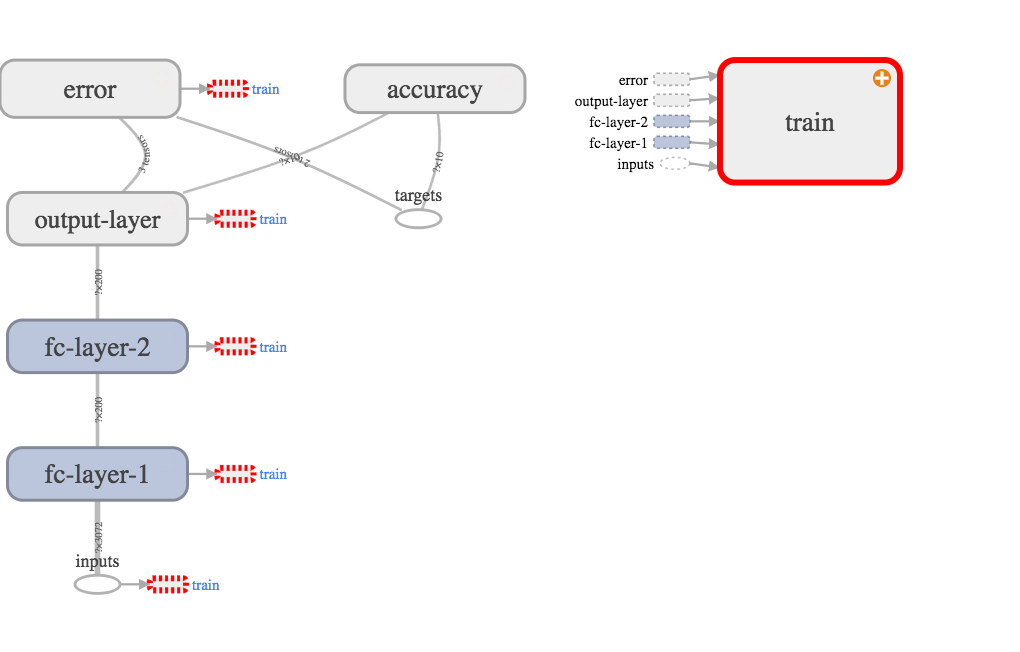
\includegraphics[width=\textwidth]{model_1}
	\caption{Showing a visual representation of the model used, from TensorBoard.}
	\label{part1-model}
	\centering
\end{figure}

\subsection{The Training}

The model was trained for 40 epochs, or 32,000 steps, with batch size of 50, in all three experiments. The \texttt{AdamOptimizer} was used as the default optimizer, with a learning rate of 0.01. The Summary Operator from TensorFlow was used to record the data from the experiments. The training data was recorded every step, whereas the validation data was recorded every 100 steps.

\subsection{The Experiments}


\subsubsection{Activation Functions}

Four activation functions were compared. The logistic sigmoid $f(x)=\frac{1}{1+e^{-x}}$, the hyperbolic tangent $f(x)=tanh(x)$ the rectified linear (ReLu) $f(x)=max(0,x)$ and the exponential linear unit (ELU):

\begin{equation} \label{eq:elu}
f(x) = \begin{cases}
x &\text{if $x >$ 0}\\ \alpha (\text{exp}(x) - 1) &\text{if  $x \leq$ 0}
\end{cases}
\end{equation}

where \(\alpha\) is a hyperparameter that decides the range of negative values for which the activation function saturates.

\begin{figure}[h]
	\centering
	\begin{tikzpicture}
	\begin{axis}[
	width=0.4\textwidth,
	axis lines = left,
	xlabel = $x$,
	ylabel = {$f(x)$},
	xmin=-4, xmax=4,
	ymin=-2, ymax=3,
	]
	\addplot[color=red]{max(0, x)};
	\end{axis}
	\end{tikzpicture}
	\begin{tikzpicture}
	\begin{axis}[
	width=0.4\textwidth,
	axis lines = left,
	xlabel = $x$,
	ylabel = {$f(x)$},
	xmin=-4, xmax=4,
	ymin=-2, ymax=3,
	]
	\addplot[color=blue]{tanh(x)};
	\end{axis}
	\end{tikzpicture}
	\begin{tikzpicture}
	\begin{axis}[
	width=0.4\textwidth,
	axis lines = left,
	xlabel = $x$,
	ylabel = {$f(x)$},
	xmin=-4, xmax=4,
	ymin=-2, ymax=3,
	]
	\addplot[color=brown]{1/(1+e^(-x))};
	\end{axis}
	\end{tikzpicture}
	\begin{tikzpicture}
	\begin{axis}[
	width=0.4\textwidth,
	axis lines = left,
	xlabel = $x$,
	ylabel = {$f(x)$},
	xmin=-4, xmax=4,
	ymin=-2, ymax=3,
	]
	\addplot[color=green, domain=-4:0]{e^(x)-1};
	\addplot[color=green, domain=0:4]{x};
	\end{axis}
	\end{tikzpicture}
	\caption{Showing the plots of the activation functions. Top Left: Relu. Top Right: Tanh. Bottom Light: Sigmoid. Bottom Right: ELU}
	\label{part1-plots}
\end{figure}

Both the hyperbolic tangent and the sigmoid functions compress their input values between (-1, 1) and (0, 1) respectively. A result of such saturation will cause their gradients to approach zero, which means smaller parameter changes and slower training. Two key differences between the two are that the hyperbolic tangent allows for both positive and negative outputs, and that the hyperbolic tangent is centered around zero. The sigmoid transformation function is centered around 0.5, which is not ideal when training models.

The ReLu transformation function looks and behaves quite differently from the two before mentioned alternatives, see Figure \ref{part1-plots}. The ReLu function has a constant gradient of 1 for activations greater than zero, and it will not suffer from diminishing gradients. It can however kill all the units, by responding to everything with 0. Furthermore, as it is unbounded, it will be more sensitive to learning rates than the sigmoid and hyperbolic tangent.

In addition to ReLu, the Exponential Linear Unit (ELU), was also tested. Although their   Unlike ReLU, the ELU responds to negative values, which pushes the mean of the activations closer to zero. Mean activations that are closer to zero enable faster learning as they bring the gradient closer to the natural gradient  \cite{elu}.

The four activation functions were used in turn to train the three-layer model presented above. The only difference, the new activation function would override the default (ReLu) non-linearity. 

\subsubsection{Hidden Layers}

depths 1 2 4 5
widths 50 100 200 400


\subsubsection{Learning Rate Schedules}

The third experiment investigates the implementation of a time-dependent learning rate schedule. This report uses an exponential learning rate schedule  
\begin{equation} \label{eq:1}
\eta(t) = \eta_{0} \gamma ^{(t / t_{decay})}
\end{equation}
where \(\eta(t)\) is the learning rate after t steps, \(\eta_{0}\) the initial learning rate and \(\gamma\) is the decay rate. \(t_{decay}\) is the number of steps required for one decay-cycle. The value of \(\gamma\) and \(t_{decay}\) determine the rate of decay of the learning rate. 

The learning schedule was implemented using already built functionality from TensorFlow. The optimiser updates the step, which changes the learning rate, which goes back into the optimiser.  The tf.train.exponential\_decay

\begin{figure}[h]
	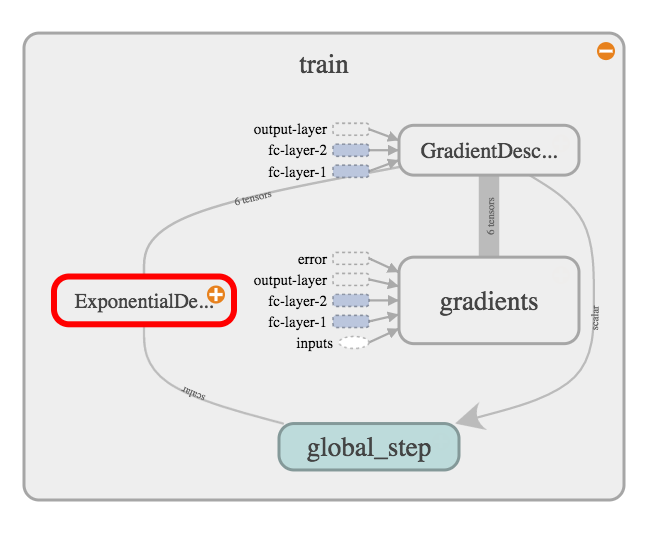
\includegraphics[width=\textwidth]{model_2}
	\caption{Showing a visual representation of the learning rate schedule, from TensorBoard.}
	\label{model_2}
	\centering
\end{figure}

The decay rate and the decay steps were only changed during some initial testing, and were set to 0.96 and 10,000 respectively. The initial learning rates used were 0.02, 0.03, 0.05, 0.07 and 0.1. 

\section{Results and Discussion}

\subsection{Activation Functions}

After the model was trained with all the activation functions, the ELU performed significantly better than the other activation functions. The final classification error for ELU was 0.96, whereas the hyperbolic tangent performed worst with a final classification error of 1.58, see Figure \ref{res-activ}. The training with ReLu and sigmoid showed similar results. 


\begin{figure}[h]
	\centering
	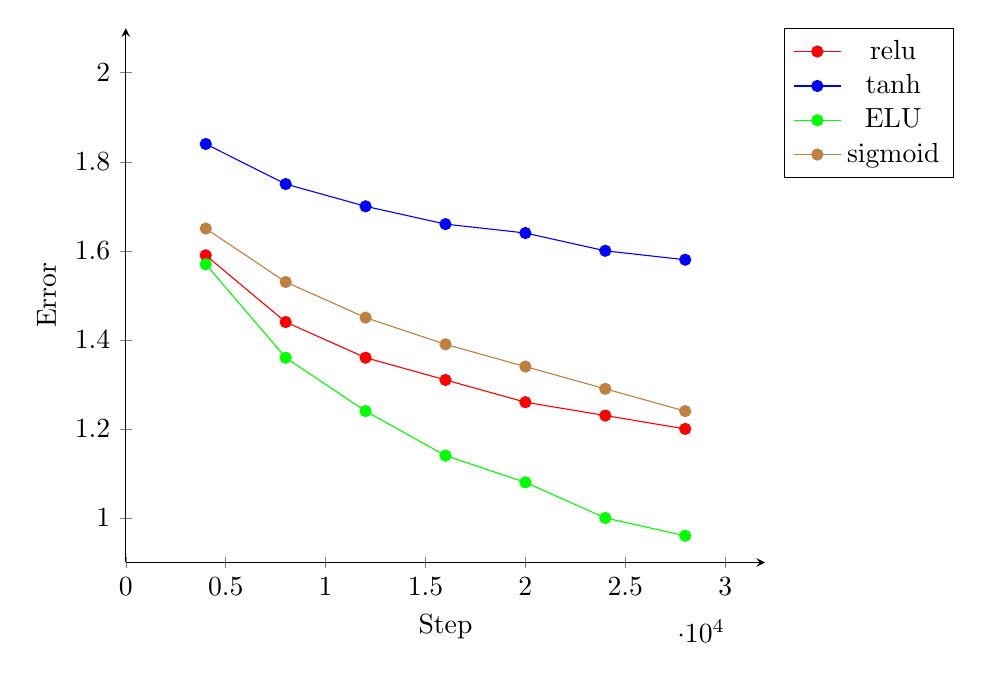
\begin{tikzpicture}
	\begin{axis}[
	width=0.8\textwidth,
	axis lines = left,
	xlabel = {Step},
	ylabel = {Error},
	xmin=0, xmax=32000,
	ymin=0.9, ymax=2.1,
	legend pos=outer north east
	]
		\addplot[color=red,mark=*]
	coordinates {
		(4000, 1.59)(8000, 1.44)(12000, 1.36)(16000, 1.31)(20000, 1.26)(24000, 1.23)(28000, 1.2)
	};
	\addlegendentry{relu};
	\addplot[color=blue,mark=*]
	coordinates {
	(4000, 1.84)(8000, 1.75)(12000, 1.7)(16000, 1.66)(20000, 1.64)(24000, 1.6)(28000, 1.58)
	};
	\addlegendentry{tanh};
	\addplot[color=green,mark=*]
	coordinates {
	(4000, 1.57)(8000, 1.36)(12000, 1.24)(16000, 1.14)(20000, 1.08)(24000, 1.0)(28000, 0.96)
};
	\addlegendentry{ELU};
	
	\addplot[color=brown,mark=*]
	coordinates {
	(4000, 1.65)(8000, 1.53)(12000, 1.45)(16000, 1.39)(20000, 1.34)(24000, 1.29)(28000, 1.24)
};
	\addlegendentry{sigmoid};
	
	\end{axis}
	\end{tikzpicture}
	
	\caption{Showing the evolution of the error function values across the training steps, for the different activation functions.}
	\label{res-activ}
\end{figure}

Based on the results presented here, it is clear that the ELU activation function outperformed the other three. As the first use of the ELU was published quite recently, it is interesting to how well the it works. Although the network used in this experiment was quite simple, the findings are consistent with those of the original publishers \cite{elu}. 



 hyperbolic tangent should be chosen before the sigmoid transformation function. The sigmoid and the tanh have similar shapes, and both suffer from the same problem of diminishing gradient. Therefore, if the hyperbolic tangent produces significantly better results, there should not be any good reasons to use the sigmoid over tanh (when training a similar model to the one used in these trials).

The ReLu and the hyperbolic tangent performed very similarly. Having to choose between the two is more difficult, but taking into account that the ReLu is computationally more efficient, that should break the tie. However, in other scenarios with different models or learning rules, an initial trial using both non-linear functions is advisable.

\begin{table}[]
	\centering
	\caption{Displaying the final classification accuracies for the activation functions.}
	\label{part1-table}
	\begin{tabular}{@{}lcc@{}}
		\toprule
		\multicolumn{1}{c}{} & Final training set accuracy & Final validation set accuracy \\ \midrule
		ELU & 0.669 & 0.505 \\
		ReLu & 0.553 & 0.483 \\
		Sigmoid & 0.537 & 0.481 \\
		Tanh & 0.472 & 0.401 \\ \bottomrule
	\end{tabular}
\end{table}


\subsection{Learning Rate Schedules}



\begin{figure}[h]
	\centering
	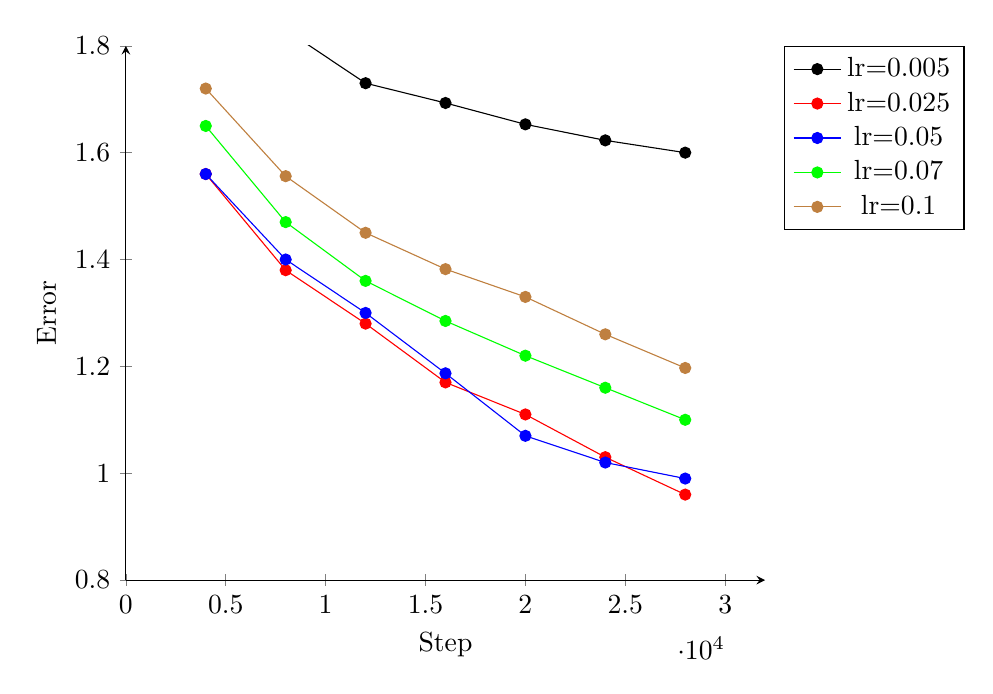
\begin{tikzpicture}
	\begin{axis}[
	width=0.8\textwidth,
	axis lines = left,
	xlabel = {Step},
	ylabel = {Error},
	xmin=0, xmax=32000,
	ymin=0.8, ymax=1.8,
	legend pos=outer north east
	]
	\addplot[color=black,mark=*]
	coordinates {
		(4000, 1.93)(12000, 1.73)(16000, 1.693)(20000, 1.653)(24000, 1.623)(28000, 1.6)
	};
	\addlegendentry{lr=0.005};
	\addplot[color=red,mark=*]
	coordinates {
		(4000, 1.56)(8000, 1.38)(12000, 1.28)(16000, 1.17)(20000, 1.11)(24000, 1.03)(28000, 0.96)
	};
	\addlegendentry{lr=0.025};
	\addplot[color=blue,mark=*]
	coordinates {
		(4000, 1.56)(8000, 1.4)(12000, 1.3)(16000, 1.187)(20000, 1.07)(24000, 1.02)(28000, 0.99)
	};
	\addlegendentry{lr=0.05};
	\addplot[color=green,mark=*]
	coordinates {
		(4000, 1.65)(8000, 1.47)(12000, 1.36)(16000, 1.285)(20000, 1.22)(24000, 1.16)(28000, 1.1)
	};
	\addlegendentry{lr=0.07};
	
	\addplot[color=brown,mark=*]
	coordinates {
		(4000, 1.72)(8000, 1.556)(12000, 1.45)(16000, 1.382)(20000, 1.33)(24000, 1.26)(28000, 1.197)
	};
	\addlegendentry{lr=0.1};
	
	\end{axis}
	\end{tikzpicture}
	
	\caption{Showing the evolution of the error function values across the training steps, for some of the initial learning rates.}
	\label{res-sch}
\end{figure}

\subsection{Hidden layers}

write here

\begin{figure}[h]
	\centering
	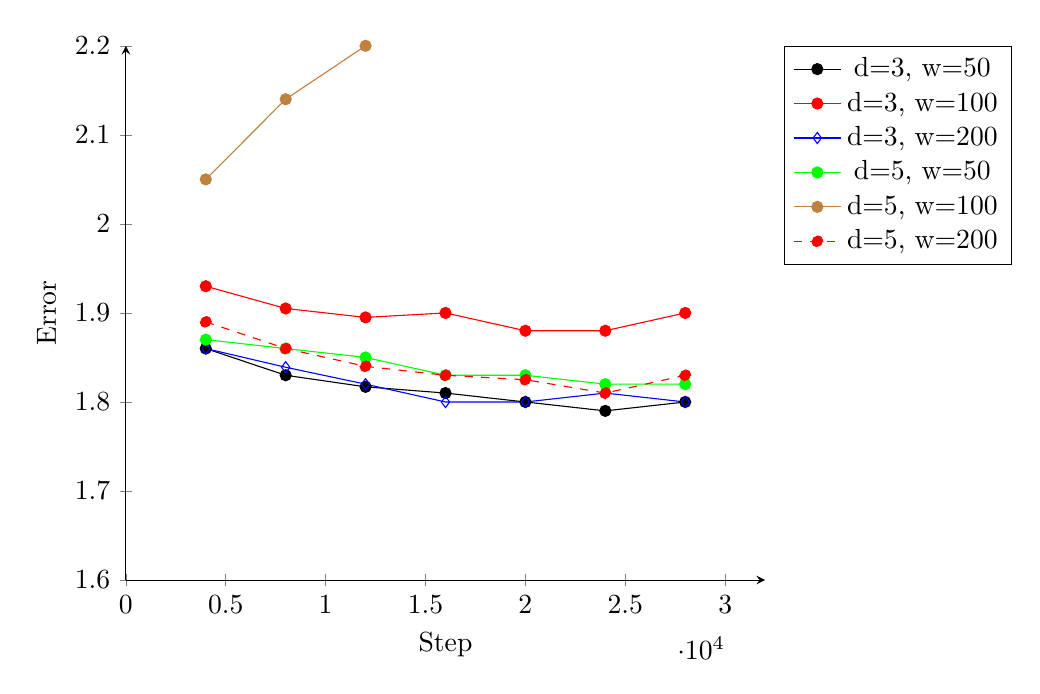
\begin{tikzpicture}
	\begin{axis}[
	width=0.8\textwidth,
	axis lines = left,
	xlabel = {Step},
	ylabel = {Error},
	xmin=0, xmax=32000,
	ymin=1.6, ymax=2.2,
	legend pos=outer north east
	]
	\addplot[color=black,mark=*]
	coordinates {
	(4000, 1.86)(8000, 1.83)(12000, 1.817)(16000, 1.81)(20000, 1.8)(24000, 1.79)(28000, 1.8)
	};
	\addlegendentry{d=3, w=50};
	\addplot[color=red,mark=*]
	coordinates {
		(4000, 1.93)(8000, 1.905)(12000, 1.895)(16000, 1.9)(20000, 1.88)(24000, 1.88)(28000, 1.9)
	};
	\addlegendentry{d=3, w=100};
\addplot[color=blue,mark=diamond]
coordinates {
	(4000, 1.86)(8000, 1.839)(12000, 1.82)(16000, 1.8)(20000, 1.8)(24000, 1.81)(28000, 1.8)
};
	\addlegendentry{d=3, w=200};
\addplot[color=green,mark=*]
coordinates {
	(4000, 1.87)(8000, 1.86)(12000, 1.85)(16000, 1.83)(20000, 1.83)(24000, 1.82)(28000, 1.82)
};
	\addlegendentry{d=5, w=50};
\addplot[color=brown,mark=*]
coordinates {
	(4000, 2.05)(8000, 2.14)(12000, 2.2)(16000, 2.24)(20000, 2.29)(24000, 2.3)(28000, 2.304)
};
	\addlegendentry{d=5, w=100};
\addplot[dashed, color=red,mark=*]
coordinates {
	(4000, 1.89)(8000, 1.86)(12000, 1.84)(16000, 1.83)(20000, 1.825)(24000, 1.81)(28000, 1.83)
};
	\addlegendentry{d=5, w=200};
	\end{axis}
	\end{tikzpicture}
	
	\caption{Showing the evolution of the error function values across the training steps, for some of the initial learning rates.}
	\label{res-hidden}
\end{figure}

\section{Conclusion}

longer trials

\section{Future Work}

Convolutional neural network, drop out, max pool
Continue to investigate ELU, in more complex models.

\clearpage
\medskip
\bibliographystyle{IEEEtran}
\bibliography{ref.bib}

\end{document}
